\chapter{Classification}\label{ml}

Previously, Chapters \ref{gle} and \ref{sce} demonstrate that both \gls{gle} and \gls{sce} contributed to characterising the cancer mutagenesis patterns. Chapter \ref{gle} shows that the smooth representation of GLE was better at discriminating cancers than the bin representation. Chapter \ref{sce} shows evidence that there is an informational advantage in exploiting the bases beyond 3-mers, namely flanking positions -2 and +2 with respect to the substitutions. 

Nonetheless, to manipulate the information from GLE and SCE, they have to be represented correctly. A sensible instinct is that a more suitable representation of a feature gives higher accuracy than a less suitable representation. This chapter acts as both an application and a validation for chapters \ref{gle} and \ref{sce}. In particular, section \ref{ml:gle} shows that smoothing GLE was a better representation than binning it. Section \ref{ml:sce} shows that currently strand symmetric 3-mer was the preferable representation of SCE. Additionally, section \ref{ml:both} demonstrates we can combine two factors with different units, like GLE and SCE, in a joint model in an attempt to further improve accuracy and to weigh the importance of each in the presence of the other.

While each of the next sections works on different data inputs, all sections follow the same procedures for training the classifier (Methods \ref{methods:ml_workflow}). Briefly, a small proportion of data was set aside as a test set, which was eventually used to evaluate model performance.

\section{Classifiers based on GLE}\label{ml:gle}
This section seeks to identify the best approach to extract information from GLE for cancer prediction. Specifically, similar to section \ref{gle:bootstrap} of Chapter \ref{gle}, I trialled the bin \textit{v.s.} smooth representations together with the Euclidean \textit{v.s.} Wasserstein distances. Again, the conventional bin representation counts mutations in discrete segments of the genome while the smooth representation computes the density of genomic locations based on how dense mutations are distributed in the neighbourhood. The Euclidean distance between two vectors aggregates the differences between points at the same coordinates on the two vectors while the Wasserstein distance allows comparing points at different coordinates. More detailed comparisons between the two representations and distance measures can be found in Methods \ref{methods:bootstrap}. For each representation and distance, I trained a KNN classifier with $\frac{1}{10}$ of the donors being used as the test set. Comparing the observations in the test set to the predictions made by the classifier allowed calculating the accuracy measure $F1$, which takes any values from 0 to 1. I iterated the training procedures 10 times to estimate the range of the $F1$ scores obtained from these approaches. $F1$ was chosen as the accuracy measure as it takes into consideration both sensitivity and specificity. Details about the training procedures can be found in Methods \ref{methods:ml_workflow}.

The results are summarised in Figure \ref{fig:f1_gle}. For the Euclidean distance, the smooth representation was much better than the bin approach in predicting cancers ($F1$ of 0.58 \textit{v.s.} 0.29). This is also very clear when inspecting the confusion matrices (Figure \ref{fig:confusion_bin_euclidean} \textit{v.s.} \ref{fig:confusion_smooth_euclidean}), where many more observations lay on the diagonals (indicating correct predictions) for the smooth representation compared to the bin representation. This is consistent with the bootstrap results from section \ref{gle:bootstrap}, where the difference in GLE between cancers was more significant for the smooth representation than the bin representation. For the Wasserstein distance, the difference between the smooth and bin approach was not obvious ($F1$ of 0.50 \textit{v.s} 0.57; Figure \ref{fig:f1_gle} and \ref{fig:apdx_ml_gle}). Besides, the $F1$ scores for both representations with the Wasserstein distance were about the same as that for the smooth representation with the Euclidean distance. This suggests that the properties of the Wasserstein distance allows it to alleviate the pitfalls introduced by the bin representation, which will be discussed in details in Section \ref{discussion:gle} of Chapter \ref{discussion}. 

\begin{figure}[htbp]
    \begin{subfigure}{.5\textwidth}
    \centering
    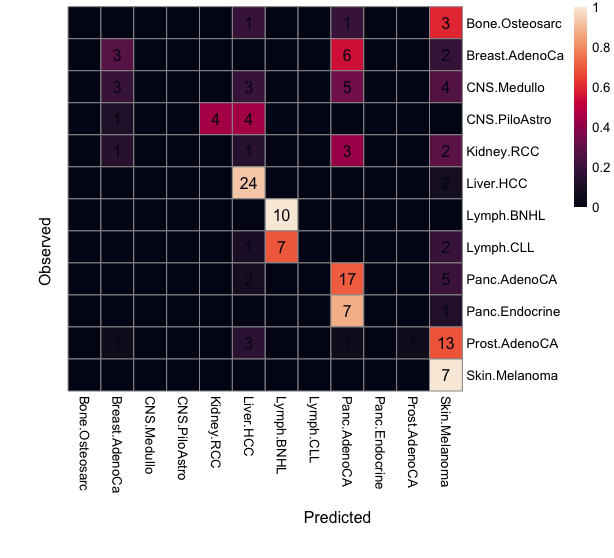
\includegraphics[width=\textwidth,height=0.9\textwidth]{graphics/confusion_matrix_bins_euclidean.png}
    \caption{Bin/Euclidean}
    \label{fig:confusion_bin_euclidean}
    \end{subfigure}
    ~
    \begin{subfigure}{.5\textwidth}
    \centering
    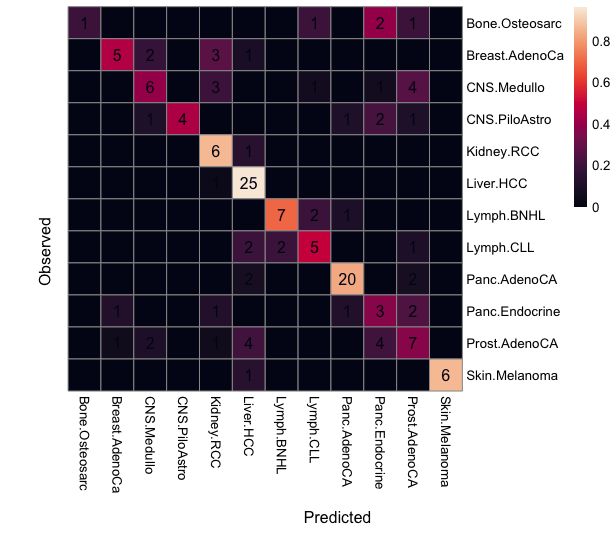
\includegraphics[width=\textwidth,height=0.9\textwidth]{graphics/confusion_matrix_smooth_euclidean.png}
    \caption{Smoothing/Euclidean}
    \label{fig:confusion_smooth_euclidean}
    \end{subfigure} \\
    \vspace{0.5cm}
    
    \begin{subfigure}{0.5\textwidth}
    \centering
    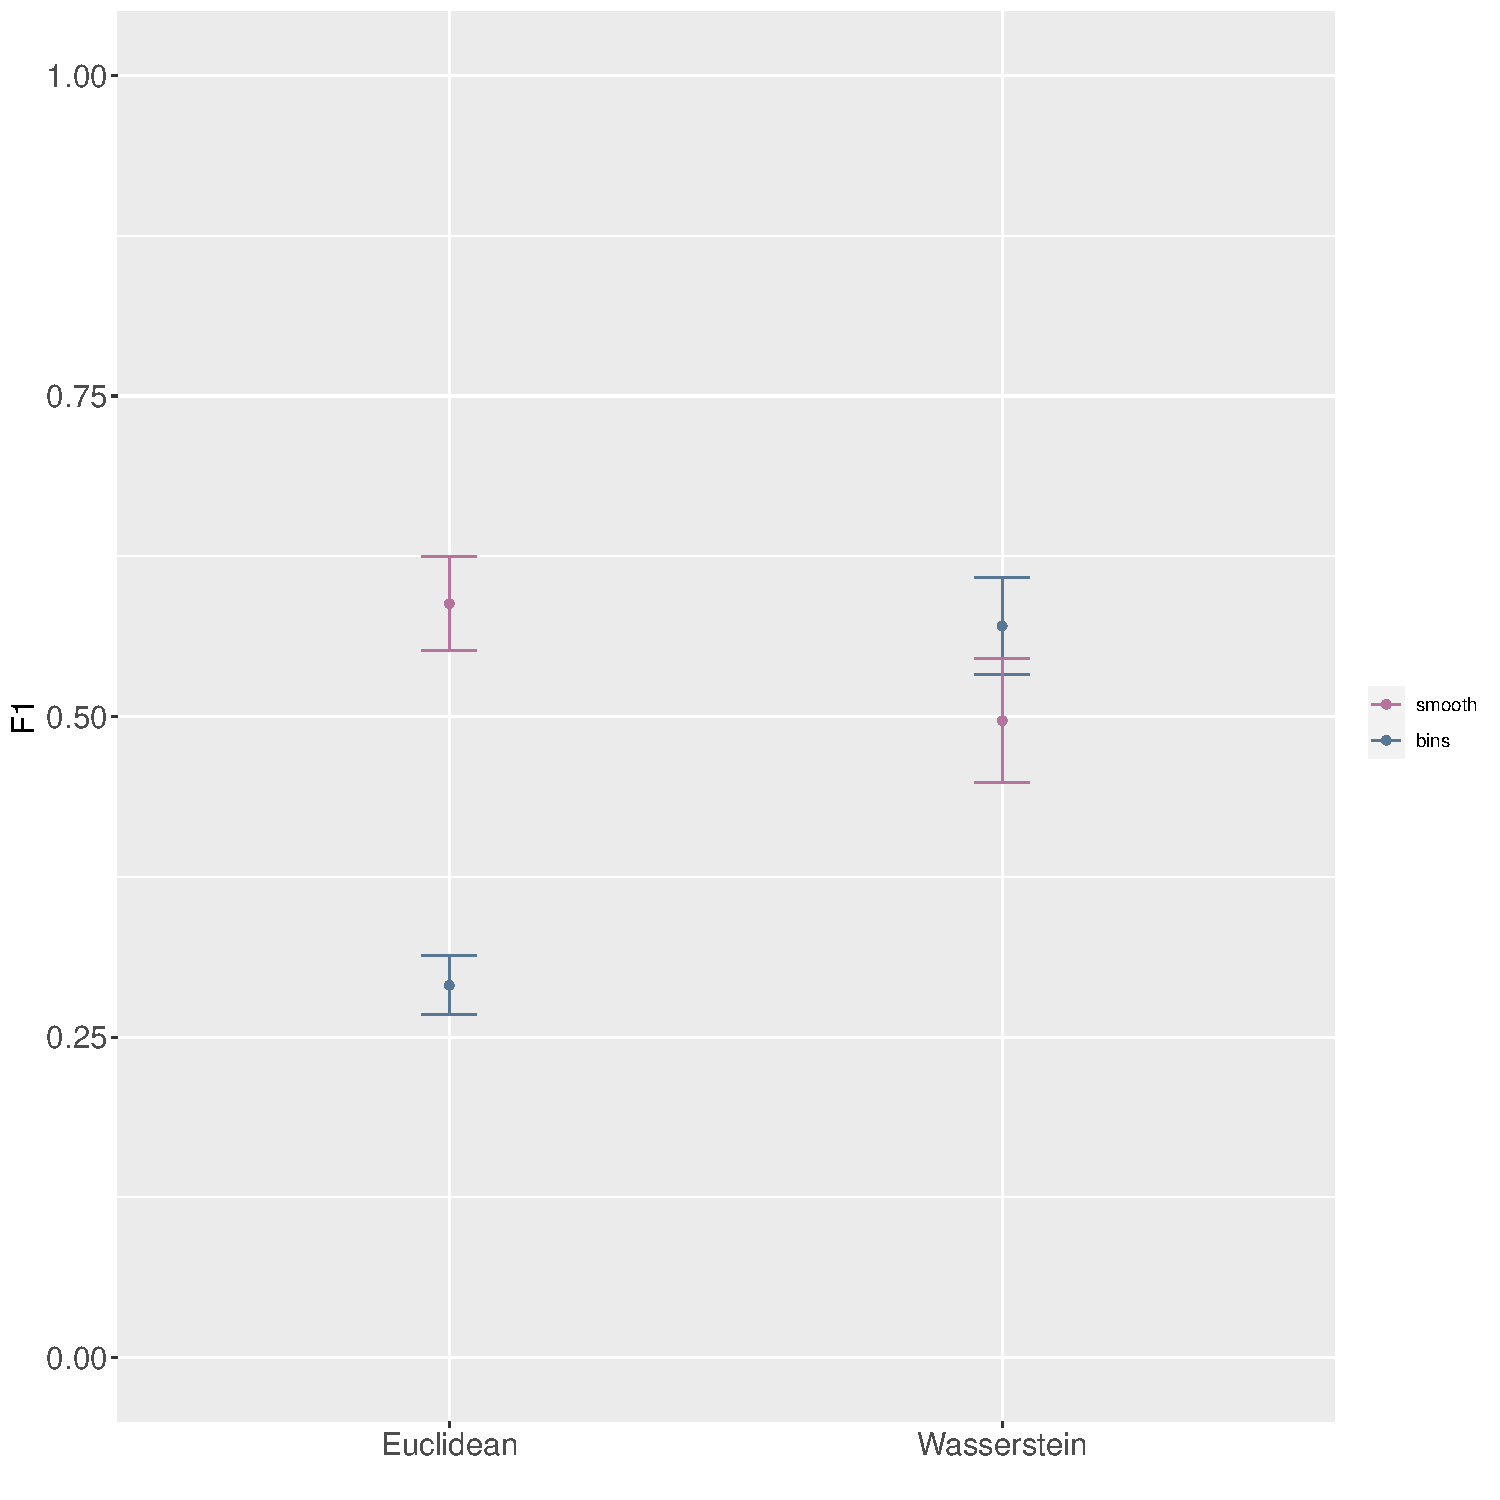
\includegraphics[scale=0.8]{graphics/f1_gle.pdf}
    \caption{F1 summary}
    \label{fig:f1_gle}
    \end{subfigure}
    
    
    \caption{\textbf{Smoothing was more accurate than binning for Euclidean distance, the difference between two representations was unclear for Wasserstein}. For each combination of representation/metric, I iterated the training procedures 10 times. Here, a representative confusion matrix, coloured by the percentage of predicted values over row total, is shown for (a) Bin/Euclidean, (b) Smooth/Euclidean. (c) shows the means of $F1$ for all representations/measures, the error bars are the standard errors for the iterated $F1$'s.}
    \label{fig:ml_gle}
\end{figure}

\section{Classifiers based on SCE}\label{ml:sce}

\subsection{3-mer was the most accurate sequence context size}
To train a classifier based on SCE, I experimented with incorporating the flanking bases to the mutation composition, including the context sizes of 1-mer, 3-mer and 5-mer, where 1-mer is the base substitution without any context. For each donor, the vector used to represent SCE was simply the counts of mutations with flanking bases incorporated, divided by the total number of mutations. The detailed representation is described in Methods \ref{methods:ml_sce}, summarised in Figure \ref{fig:sce_counts}. In parallel, due to the strand symmetry observed in Chapter \ref{sce}, I also trialled imposing different levels of symmetry to SCE. These include asymmetry (no symmetry, \textit{i.e.} the normal count vector), semi-symmetry (reverse complementary mutations being counted as the same category) and full-symmetry (reverse complementary mutations being counted as the same category and flanking bases restricted to be A and C). Out of three levels of symmetry, the semi-symmetric representation was the commonly used method, as introduced in Section \ref{intro:sce}; the fully-symmetric representation was an experiment with the length of the SCE vectors. Methods \ref{methods:ml_sce} and Table \ref{tab:sce_symmetric} provide a more detailed depiction of the representations for the three levels of strand symmetry. The algorithm and the accuracy measure recruited for SCE were KNN and $F1$, respectively, with Jensen-Shannon used as the distance measure. 

Figure \ref{fig:f1_sce} shows the $F1$ for different $k$-mer sizes and different levels of strand symmetry. The corresponding confusion matrices can be found in Figure \ref{fig:apdx_ml_sce}. In general, SCE was more accurate than GLE, with 3-mer being the best representation ($F1=0.83$). Asymmetry and semi-symmetry performed roughly similarly, reinforcing the evidence of strand symmetry previously seen in Chapter \ref{sce}. Assuming asymmetry and semi-symmetry are equivalent, $F1$ being lower for 5-mer than 3-mer but higher for semi-symmetry than asymmetry is very curious. Combined with the observation in section \ref{sce:nbr} of Chapter \ref{sce} that there was information in the outer positions -2 and +2, this suggests there is an impact of splitting up mutation counts into too many elements in 5-mers (Methods Table \ref{tab:sce_symmetric}). However, the length of the input vector was not the only determinant of accuracy as the fully symmetric representation, despite its short vector, severely dropped in accuracy. This suggests that the fully symmetric representation introduced noise to the data.

\begin{figure}[h!]
    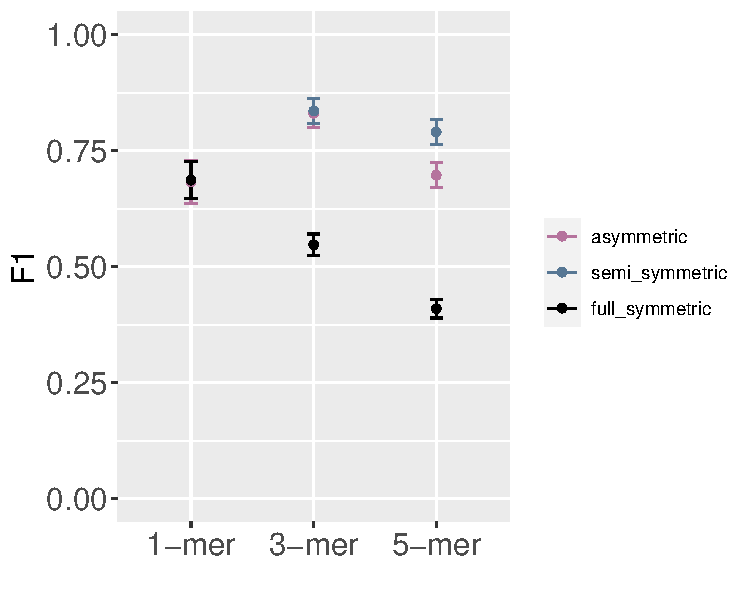
\includegraphics[scale=0.75]{graphics/f1_sce.pdf}
    \caption{\textbf{SCE classifiers using the 3-mer context  were the most accurate}. For each combination of representation/metric, I iterated the training procedures of the KNN classifier 10 times using Jensen-Shannon distance. The performance of the classifier was computed based on a previously held out test data set and reported as confusion matrices and $F1$'s. The y-axis is the means of $F1$ for 1-mer, 3-mer \& 5-mer and asymmetry, semi-symmetry \& full-symmetry; the error bars are the standard errors for the iterated $F1$’s. The corresponding confusion matrices are shown in Figure \ref{fig:apdx_ml_sce}.}
    \label{fig:f1_sce}
\end{figure}


\subsection{Dissecting 5-mer into submotifs could potentially improve accuracy}
Suspecting that the poor performance of 5-mer was due to the long vector that represented it, I tried splitting up 5-mers into smaller vectors that incorporate fewer flanking positions. For instance, for 2-submotifs, I split the long 5-mer vector into 4 shorter vectors that only involved 2 positions, the base substitution and one flanking position. Similarly, 3-submotifs are 3 short vectors, each involving the base substitution and two flanking positions. Each component short vectors provided a pairwise distance matrix and the average of the resulting distance matrices was input to the KNN classifier. This is described in details in Methods \ref{methods:ml_sce}. The subsequent steps were the same as the normal training procedures.

Figure \ref{fig:f1_sce_submotif} shows that the splitting did improve $F1$ compared to the original whole 5-mer vector, particularly the 3-submotif representation. The corresponding confusion matrices can be found in Figure \ref{fig:apdx_ml_submotifs}. This is very promising, but at this point it is uncertain whether it was the information from outer flanking positions or the 3-mer incorporated in the 3-motifs that drove this accuracy improvement.

\begin{figure}[h!]
    \centering
    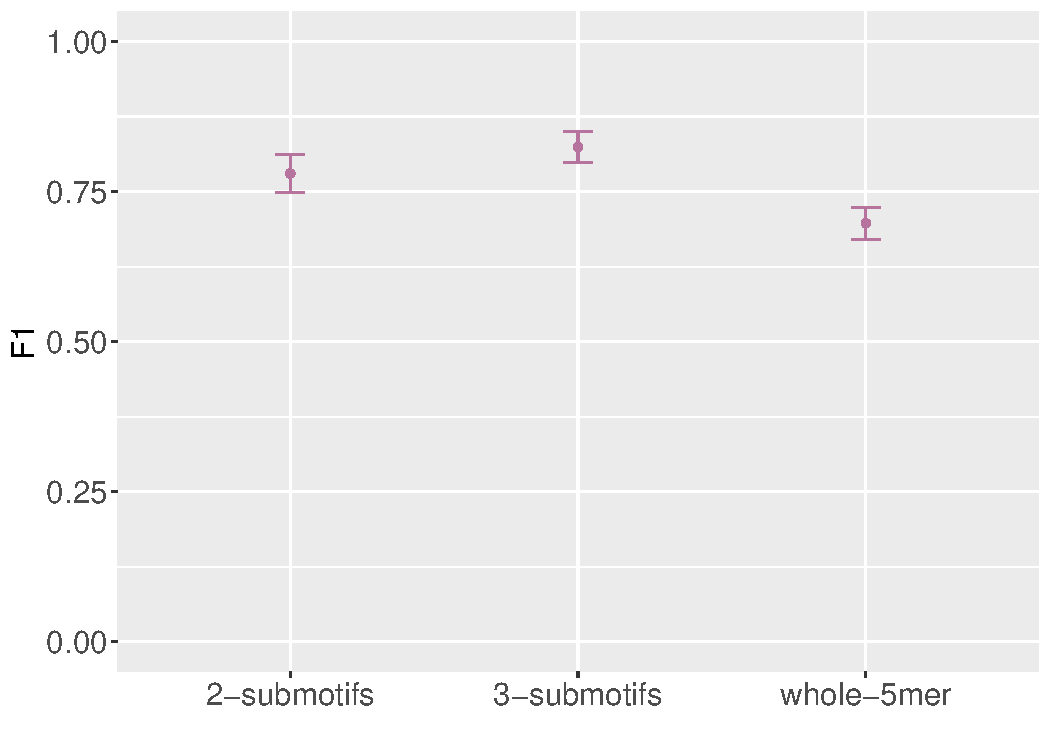
\includegraphics[scale=1]{graphics/f1_sce_submotif.pdf}
    \caption{\textbf{Dissecting 5-mer into multiple submotifs can potentially improve prediction accuracy compared to whole 5-mer}. For each combination of representation, I iterated the training procedures 10 times. The y-axis is the means of $F1$ for all representations/measures, the error bars are the standard errors for the iterated $F1$'s.}
    \label{fig:f1_sce_submotif}
\end{figure}


\section{Classifiers based on the combination of GLE and SCE}\label{ml:both}
In this section, I attempted to combine GLE and SCE to see whether the combination could improve the accuracy over each factor by itself. In terms of representation, I used two approaches, the conventional and the proposed approach. The conventional approach combined the bin representation for GLE and the semi-symmetric 3-mer representation for SCE. The proposed approach combined the smooth representation for GLE and the asymmetric 3-mer representation for SCE. For both approaches, I used the Euclidean distance for GLE and Jensen-Shannon distance for SCE. To combine GLE and SCE, I converted the distance matrices for the two factors into the kernel matrices, during which their scales and units were normalised. I then combined the kernel matrices, trialling different weights and converted the resulting kernel matrix into a joint distance matrix (details in Methods \ref{methods:ml_both}). The subsequent steps were the same as the normal training procedures.

I reported $F1$ in Figure \ref{fig:f1_combined}. For both approaches, $F1$ improved for GLE but not SCE. In fact, the accuracy was predominated by SCE, which is particularly true for the bin/semi-symmetry combination. Since both GLE and SCE were previously normalised, the influence of SCE on $F1$ shows that it was the stronger predictor of cancers than GLE.

\begin{figure}[h!]
    \centering
    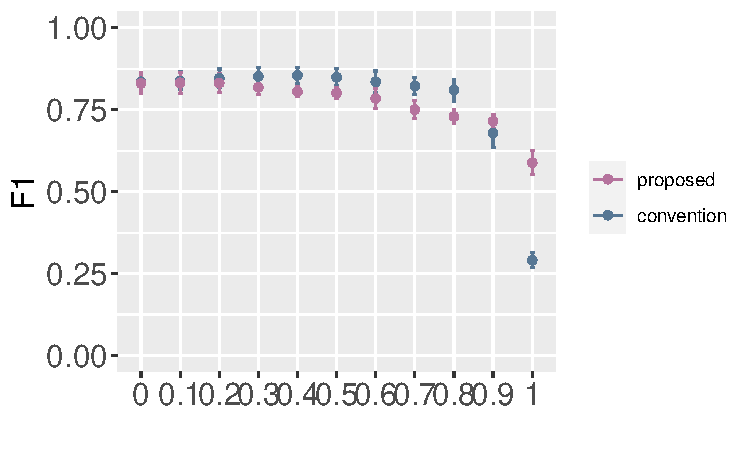
\includegraphics[scale=0.7]{graphics/f1_combined.pdf}
    \caption{\textbf{SCE was the stronger predictor of cancer prediction}. I combined GLE and SCE using two approaches: the conventional approach (bin for GLE and semi-symmetric 3-mer for SCE) and the proposed approach (smooth for GLE and asymmetric 3-mer for SCE). I used Euclidean distance for GLE and Jensen-Shannon distance for SCE. The x-axis is the weight given to GLE $g$, the weight given to SCE is accordingly $1-g$. For each weight combination, I iterated the training procedures 10 times. The y-axis is the means of $F1$ for all representations, the error bars are the standard errors for the iterated $F1$'s.}
    \label{fig:f1_combined}
\end{figure}


\section{Chapter summary}
In accordance with Chapters \ref{gle} and \ref{sce}, this chapter shows that both GLE and SCE are good predictors of cancers, with SCE being the stronger factor. All classifiers used the KNN algorithm with $F1$ as the measure of accuracy. Section \ref{ml:gle} shows that the smooth representation of GLE was more accurate than the bin representation. However, the Wasserstein distance had properties that allowed it to alleviate the pitfalls from the bin representation. Section \ref{ml:sce} shows that the information from flanking bases were useful for cancer classification (Jensen-Shannon distance was used). In particular, the 3-mer representation involving three positions, the base substitution and positions -1 and +1, performed best. That said, the length of the SCE vector had an impact on the performance of the classifier. This manifests in that 5-mer was less accurate than 3-mer, even though information was shown to be available in positions -2 and +2 in Chapter \ref{sce}. Besides, the accuracy for 5-mer improved when splitting it up into shorter vectors. Evidence of strand-symmetry was again present, as the semi-symmetric representation was at least as accurate as the asymmetric representation. Finally, Section \ref{ml:both} shows that SCE was the stronger predictor of cancers than GLE, because the accuracy was mostly determined by SCE even after both GLE and SCE were normalised.

